% Options for packages loaded elsewhere
\PassOptionsToPackage{unicode}{hyperref}
\PassOptionsToPackage{hyphens}{url}
%
\documentclass[
]{article}
\usepackage{amsmath,amssymb}
\usepackage{lmodern}
\usepackage{iftex}
\ifPDFTeX
  \usepackage[T1]{fontenc}
  \usepackage[utf8]{inputenc}
  \usepackage{textcomp} % provide euro and other symbols
\else % if luatex or xetex
  \usepackage{unicode-math}
  \defaultfontfeatures{Scale=MatchLowercase}
  \defaultfontfeatures[\rmfamily]{Ligatures=TeX,Scale=1}
\fi
% Use upquote if available, for straight quotes in verbatim environments
\IfFileExists{upquote.sty}{\usepackage{upquote}}{}
\IfFileExists{microtype.sty}{% use microtype if available
  \usepackage[]{microtype}
  \UseMicrotypeSet[protrusion]{basicmath} % disable protrusion for tt fonts
}{}
\makeatletter
\@ifundefined{KOMAClassName}{% if non-KOMA class
  \IfFileExists{parskip.sty}{%
    \usepackage{parskip}
  }{% else
    \setlength{\parindent}{0pt}
    \setlength{\parskip}{6pt plus 2pt minus 1pt}}
}{% if KOMA class
  \KOMAoptions{parskip=half}}
\makeatother
\usepackage{xcolor}
\usepackage[margin=1in]{geometry}
\usepackage{color}
\usepackage{fancyvrb}
\newcommand{\VerbBar}{|}
\newcommand{\VERB}{\Verb[commandchars=\\\{\}]}
\DefineVerbatimEnvironment{Highlighting}{Verbatim}{commandchars=\\\{\}}
% Add ',fontsize=\small' for more characters per line
\usepackage{framed}
\definecolor{shadecolor}{RGB}{248,248,248}
\newenvironment{Shaded}{\begin{snugshade}}{\end{snugshade}}
\newcommand{\AlertTok}[1]{\textcolor[rgb]{0.94,0.16,0.16}{#1}}
\newcommand{\AnnotationTok}[1]{\textcolor[rgb]{0.56,0.35,0.01}{\textbf{\textit{#1}}}}
\newcommand{\AttributeTok}[1]{\textcolor[rgb]{0.77,0.63,0.00}{#1}}
\newcommand{\BaseNTok}[1]{\textcolor[rgb]{0.00,0.00,0.81}{#1}}
\newcommand{\BuiltInTok}[1]{#1}
\newcommand{\CharTok}[1]{\textcolor[rgb]{0.31,0.60,0.02}{#1}}
\newcommand{\CommentTok}[1]{\textcolor[rgb]{0.56,0.35,0.01}{\textit{#1}}}
\newcommand{\CommentVarTok}[1]{\textcolor[rgb]{0.56,0.35,0.01}{\textbf{\textit{#1}}}}
\newcommand{\ConstantTok}[1]{\textcolor[rgb]{0.00,0.00,0.00}{#1}}
\newcommand{\ControlFlowTok}[1]{\textcolor[rgb]{0.13,0.29,0.53}{\textbf{#1}}}
\newcommand{\DataTypeTok}[1]{\textcolor[rgb]{0.13,0.29,0.53}{#1}}
\newcommand{\DecValTok}[1]{\textcolor[rgb]{0.00,0.00,0.81}{#1}}
\newcommand{\DocumentationTok}[1]{\textcolor[rgb]{0.56,0.35,0.01}{\textbf{\textit{#1}}}}
\newcommand{\ErrorTok}[1]{\textcolor[rgb]{0.64,0.00,0.00}{\textbf{#1}}}
\newcommand{\ExtensionTok}[1]{#1}
\newcommand{\FloatTok}[1]{\textcolor[rgb]{0.00,0.00,0.81}{#1}}
\newcommand{\FunctionTok}[1]{\textcolor[rgb]{0.00,0.00,0.00}{#1}}
\newcommand{\ImportTok}[1]{#1}
\newcommand{\InformationTok}[1]{\textcolor[rgb]{0.56,0.35,0.01}{\textbf{\textit{#1}}}}
\newcommand{\KeywordTok}[1]{\textcolor[rgb]{0.13,0.29,0.53}{\textbf{#1}}}
\newcommand{\NormalTok}[1]{#1}
\newcommand{\OperatorTok}[1]{\textcolor[rgb]{0.81,0.36,0.00}{\textbf{#1}}}
\newcommand{\OtherTok}[1]{\textcolor[rgb]{0.56,0.35,0.01}{#1}}
\newcommand{\PreprocessorTok}[1]{\textcolor[rgb]{0.56,0.35,0.01}{\textit{#1}}}
\newcommand{\RegionMarkerTok}[1]{#1}
\newcommand{\SpecialCharTok}[1]{\textcolor[rgb]{0.00,0.00,0.00}{#1}}
\newcommand{\SpecialStringTok}[1]{\textcolor[rgb]{0.31,0.60,0.02}{#1}}
\newcommand{\StringTok}[1]{\textcolor[rgb]{0.31,0.60,0.02}{#1}}
\newcommand{\VariableTok}[1]{\textcolor[rgb]{0.00,0.00,0.00}{#1}}
\newcommand{\VerbatimStringTok}[1]{\textcolor[rgb]{0.31,0.60,0.02}{#1}}
\newcommand{\WarningTok}[1]{\textcolor[rgb]{0.56,0.35,0.01}{\textbf{\textit{#1}}}}
\usepackage{graphicx}
\makeatletter
\def\maxwidth{\ifdim\Gin@nat@width>\linewidth\linewidth\else\Gin@nat@width\fi}
\def\maxheight{\ifdim\Gin@nat@height>\textheight\textheight\else\Gin@nat@height\fi}
\makeatother
% Scale images if necessary, so that they will not overflow the page
% margins by default, and it is still possible to overwrite the defaults
% using explicit options in \includegraphics[width, height, ...]{}
\setkeys{Gin}{width=\maxwidth,height=\maxheight,keepaspectratio}
% Set default figure placement to htbp
\makeatletter
\def\fps@figure{htbp}
\makeatother
\setlength{\emergencystretch}{3em} % prevent overfull lines
\providecommand{\tightlist}{%
  \setlength{\itemsep}{0pt}\setlength{\parskip}{0pt}}
\setcounter{secnumdepth}{5}
\ifLuaTeX
  \usepackage{selnolig}  % disable illegal ligatures
\fi
\IfFileExists{bookmark.sty}{\usepackage{bookmark}}{\usepackage{hyperref}}
\IfFileExists{xurl.sty}{\usepackage{xurl}}{} % add URL line breaks if available
\urlstyle{same} % disable monospaced font for URLs
\hypersetup{
  pdftitle={Análise de dados (EDA)},
  pdfauthor={Cristian Villegas},
  hidelinks,
  pdfcreator={LaTeX via pandoc}}

\title{Análise de dados (EDA)}
\author{Cristian Villegas}
\date{2023-05-18}

\begin{document}
\maketitle

{
\setcounter{tocdepth}{2}
\tableofcontents
}
\hypertarget{leitura-de-dados}{%
\section{Leitura de dados}\label{leitura-de-dados}}

\begin{Shaded}
\begin{Highlighting}[]
\FunctionTok{library}\NormalTok{(tidyverse)}
\FunctionTok{library}\NormalTok{(hnp)}

\NormalTok{dados }\OtherTok{\textless{}{-}} \FunctionTok{read.csv}\NormalTok{(}\StringTok{"Arthritis.txt"}\NormalTok{, }\AttributeTok{sep=}\StringTok{""}\NormalTok{, }
                  \AttributeTok{stringsAsFactors=}\ConstantTok{TRUE}\NormalTok{)}

\NormalTok{dados}\SpecialCharTok{$}\NormalTok{id}\OtherTok{\textless{}{-}} \DecValTok{1}\SpecialCharTok{:}\FunctionTok{nrow}\NormalTok{(dados)}

\NormalTok{dados}\OtherTok{\textless{}{-}} \FunctionTok{tibble}\NormalTok{(dados)}
\NormalTok{dados}
\end{Highlighting}
\end{Shaded}

\begin{verbatim}
## # A tibble: 51 x 9
##    Sex     Age Group Week0 Week1 Week5 Week9 Week13    id
##    <fct> <int> <fct> <int> <int> <int> <int>  <int> <int>
##  1 M        48 A         1     1     1     1      1     1
##  2 M        29 A         1     1     1     1      1     2
##  3 M        59 P         1     1     1     1      1     3
##  4 F        56 P         1     1     1     1      1     4
##  5 M        33 P         1     1     1     1      1     5
##  6 M        61 P         1     1     0     1      1     6
##  7 M        63 A         0     0     1    NA     NA     7
##  8 M        57 P         1     0     1     1      1     8
##  9 M        47 P         1     1     1     0      1     9
## 10 F        42 A         0     0     1    NA      0    10
## # ... with 41 more rows
\end{verbatim}

\hypertarget{alguns-resumos-dos-dados}{%
\section{Alguns resumos dos dados}\label{alguns-resumos-dos-dados}}

\begin{Shaded}
\begin{Highlighting}[]
\NormalTok{dados }\SpecialCharTok{\%\textgreater{}\%} 
  \FunctionTok{group\_by}\NormalTok{(Sex) }\SpecialCharTok{\%\textgreater{}\%} 
  \FunctionTok{summarise}\NormalTok{( }\AttributeTok{n =} \FunctionTok{n}\NormalTok{())}
\end{Highlighting}
\end{Shaded}

\begin{verbatim}
## # A tibble: 2 x 2
##   Sex       n
##   <fct> <int>
## 1 F        13
## 2 M        38
\end{verbatim}

\begin{Shaded}
\begin{Highlighting}[]
\NormalTok{dados }\SpecialCharTok{\%\textgreater{}\%} 
  \FunctionTok{group\_by}\NormalTok{(Sex) }\SpecialCharTok{\%\textgreater{}\%} 
  \FunctionTok{summarise}\NormalTok{(}\AttributeTok{media\_Sex =} \FunctionTok{mean}\NormalTok{(Age))}
\end{Highlighting}
\end{Shaded}

\begin{verbatim}
## # A tibble: 2 x 2
##   Sex   media_Sex
##   <fct>     <dbl>
## 1 F          51.8
## 2 M          50.2
\end{verbatim}

\begin{Shaded}
\begin{Highlighting}[]
\NormalTok{dados }\SpecialCharTok{\%\textgreater{}\%} 
  \FunctionTok{group\_by}\NormalTok{(Group) }\SpecialCharTok{\%\textgreater{}\%} 
  \FunctionTok{summarise}\NormalTok{( }\AttributeTok{n =} \FunctionTok{n}\NormalTok{())}
\end{Highlighting}
\end{Shaded}

\begin{verbatim}
## # A tibble: 2 x 2
##   Group     n
##   <fct> <int>
## 1 A        27
## 2 P        24
\end{verbatim}

\begin{Shaded}
\begin{Highlighting}[]
\NormalTok{dados }\SpecialCharTok{\%\textgreater{}\%} 
  \FunctionTok{group\_by}\NormalTok{(Group) }\SpecialCharTok{\%\textgreater{}\%} 
  \FunctionTok{summarise}\NormalTok{( }\AttributeTok{media\_Age =} \FunctionTok{mean}\NormalTok{(Age))}
\end{Highlighting}
\end{Shaded}

\begin{verbatim}
## # A tibble: 2 x 2
##   Group media_Age
##   <fct>     <dbl>
## 1 A          51.0
## 2 P          50.2
\end{verbatim}

\begin{Shaded}
\begin{Highlighting}[]
\NormalTok{dados }\SpecialCharTok{\%\textgreater{}\%} 
  \FunctionTok{group\_by}\NormalTok{(Sex, Group) }\SpecialCharTok{\%\textgreater{}\%} 
  \FunctionTok{summarise}\NormalTok{( }\AttributeTok{n =} \FunctionTok{n}\NormalTok{())}
\end{Highlighting}
\end{Shaded}

\begin{verbatim}
## # A tibble: 4 x 3
## # Groups:   Sex [2]
##   Sex   Group     n
##   <fct> <fct> <int>
## 1 F     A         7
## 2 F     P         6
## 3 M     A        20
## 4 M     P        18
\end{verbatim}

\hypertarget{gruxe1ficos-de-interesse}{%
\section{Gráficos de interesse}\label{gruxe1ficos-de-interesse}}

\begin{Shaded}
\begin{Highlighting}[]
\FunctionTok{ggplot}\NormalTok{(dados, }\FunctionTok{aes}\NormalTok{(}\AttributeTok{x =}\NormalTok{ Sex)) }\SpecialCharTok{+}
  \FunctionTok{geom\_bar}\NormalTok{()}
\end{Highlighting}
\end{Shaded}

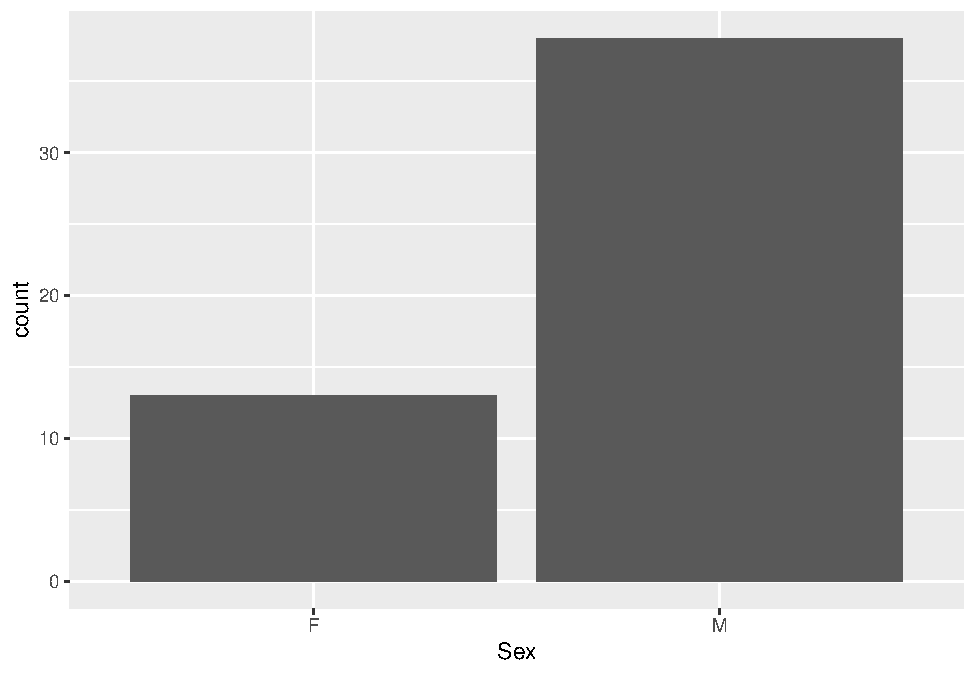
\includegraphics{EDA__files/figure-latex/unnamed-chunk-3-1.pdf}

\begin{Shaded}
\begin{Highlighting}[]
\FunctionTok{ggplot}\NormalTok{(dados, }\FunctionTok{aes}\NormalTok{(}\AttributeTok{x =}\NormalTok{ Group)) }\SpecialCharTok{+}
  \FunctionTok{geom\_bar}\NormalTok{()}
\end{Highlighting}
\end{Shaded}

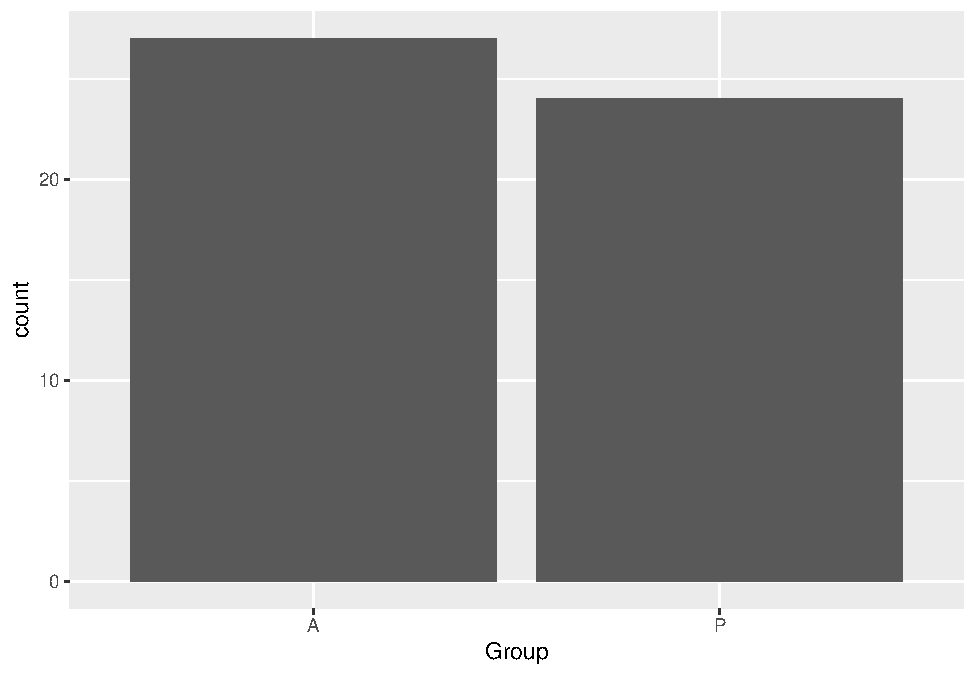
\includegraphics{EDA__files/figure-latex/unnamed-chunk-3-2.pdf}

\hypertarget{transformando-os-dados}{%
\section{Transformando os dados}\label{transformando-os-dados}}

\begin{Shaded}
\begin{Highlighting}[]
\NormalTok{dados\_longos}\OtherTok{\textless{}{-}}\NormalTok{ dados }\SpecialCharTok{\%\textgreater{}\%}
  \FunctionTok{pivot\_longer}\NormalTok{(}
    \AttributeTok{cols =} \FunctionTok{starts\_with}\NormalTok{(}\StringTok{"Week"}\NormalTok{),}
    \AttributeTok{names\_to =} \StringTok{"week"}\NormalTok{,}
    \AttributeTok{names\_prefix =} \StringTok{"Week"}\NormalTok{,}
    \AttributeTok{values\_to =} \StringTok{"Y"}\NormalTok{,}
    \AttributeTok{values\_drop\_na =} \ConstantTok{TRUE}
\NormalTok{  )}
\end{Highlighting}
\end{Shaded}

\hypertarget{gruxe1ficos-antes-de-transformar-dados}{%
\subsection{Gráficos antes de transformar
dados}\label{gruxe1ficos-antes-de-transformar-dados}}

\begin{Shaded}
\begin{Highlighting}[]
\FunctionTok{ggplot}\NormalTok{(dados\_longos, }\FunctionTok{aes}\NormalTok{(Sex, Age, }\AttributeTok{col =}\NormalTok{ Age }\SpecialCharTok{\textless{}} \DecValTok{50}\NormalTok{)) }\SpecialCharTok{+} 
  \FunctionTok{geom\_boxplot}\NormalTok{()}\SpecialCharTok{+}
  \FunctionTok{geom\_hline}\NormalTok{(}\AttributeTok{yintercept =} \DecValTok{50}\NormalTok{, }\AttributeTok{col =} \StringTok{"black"}\NormalTok{, }\AttributeTok{linetype =} \DecValTok{2}\NormalTok{)}\SpecialCharTok{+}
  \FunctionTok{theme\_minimal}\NormalTok{()}
\end{Highlighting}
\end{Shaded}

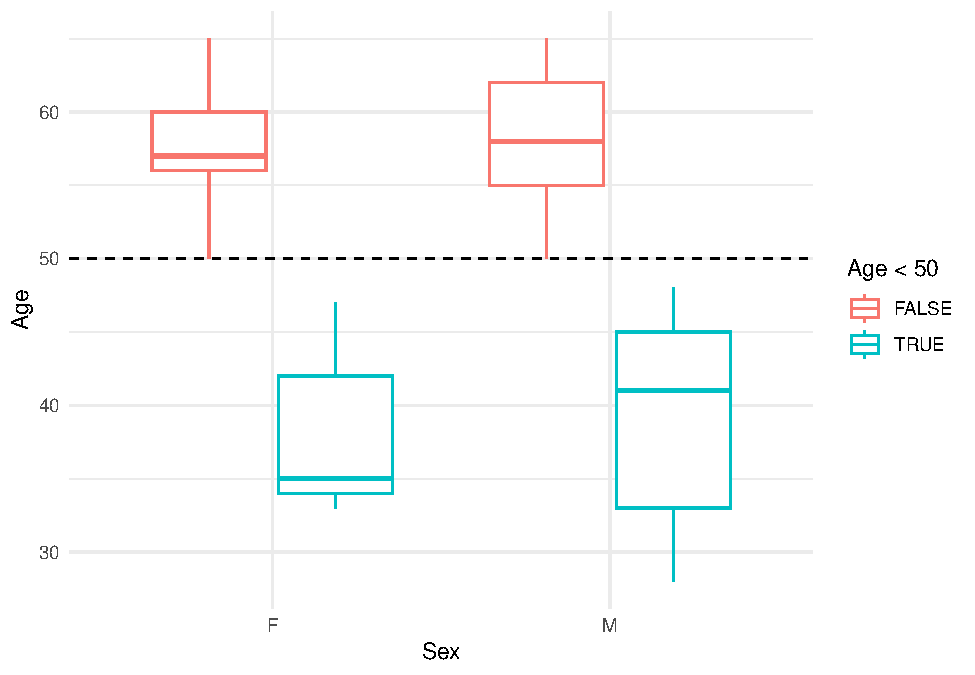
\includegraphics{EDA__files/figure-latex/unnamed-chunk-5-1.pdf}

\begin{Shaded}
\begin{Highlighting}[]
\FunctionTok{ggplot}\NormalTok{(dados\_longos, }\FunctionTok{aes}\NormalTok{(Group, Age, }\AttributeTok{col =}\NormalTok{ Age }\SpecialCharTok{\textless{}} \DecValTok{50}\NormalTok{)) }\SpecialCharTok{+} 
  \FunctionTok{geom\_boxplot}\NormalTok{()}\SpecialCharTok{+}
  \FunctionTok{geom\_hline}\NormalTok{(}\AttributeTok{yintercept =} \DecValTok{50}\NormalTok{, }\AttributeTok{col =} \StringTok{"black"}\NormalTok{, }\AttributeTok{linetype =} \DecValTok{2}\NormalTok{)}\SpecialCharTok{+}
  \FunctionTok{theme\_minimal}\NormalTok{()}
\end{Highlighting}
\end{Shaded}

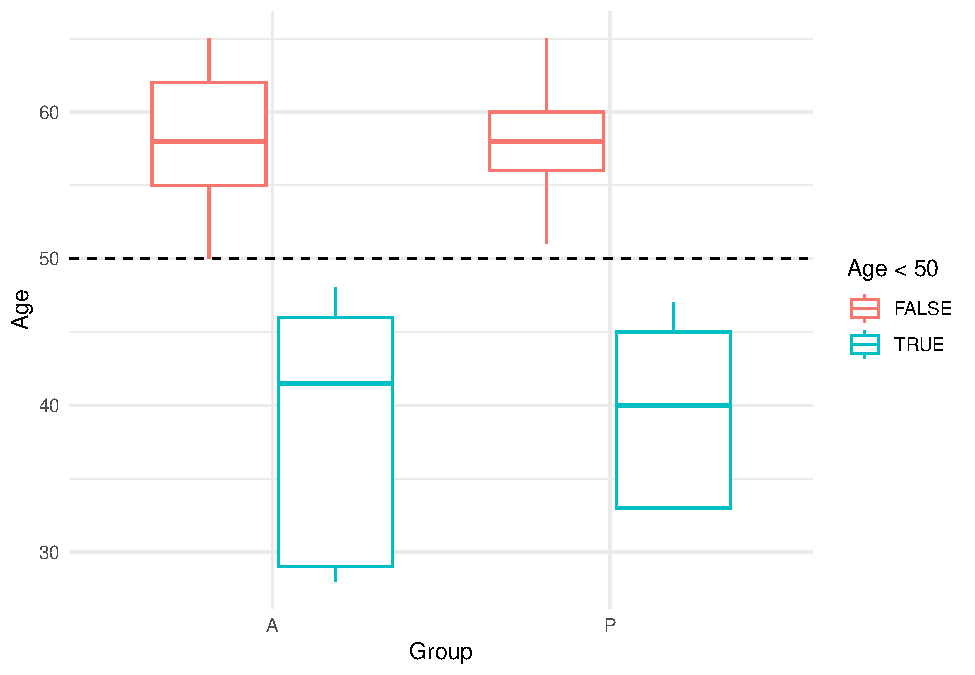
\includegraphics{EDA__files/figure-latex/unnamed-chunk-5-2.pdf}

\begin{Shaded}
\begin{Highlighting}[]
\FunctionTok{ggplot}\NormalTok{(dados\_longos, }\FunctionTok{aes}\NormalTok{(}\AttributeTok{x =}\NormalTok{ Sex, }\AttributeTok{fill =}\NormalTok{ Group)) }\SpecialCharTok{+} 
  \FunctionTok{geom\_bar}\NormalTok{(}\AttributeTok{position=}\FunctionTok{position\_dodge}\NormalTok{())}\SpecialCharTok{+}
  \FunctionTok{theme\_minimal}\NormalTok{()}
\end{Highlighting}
\end{Shaded}

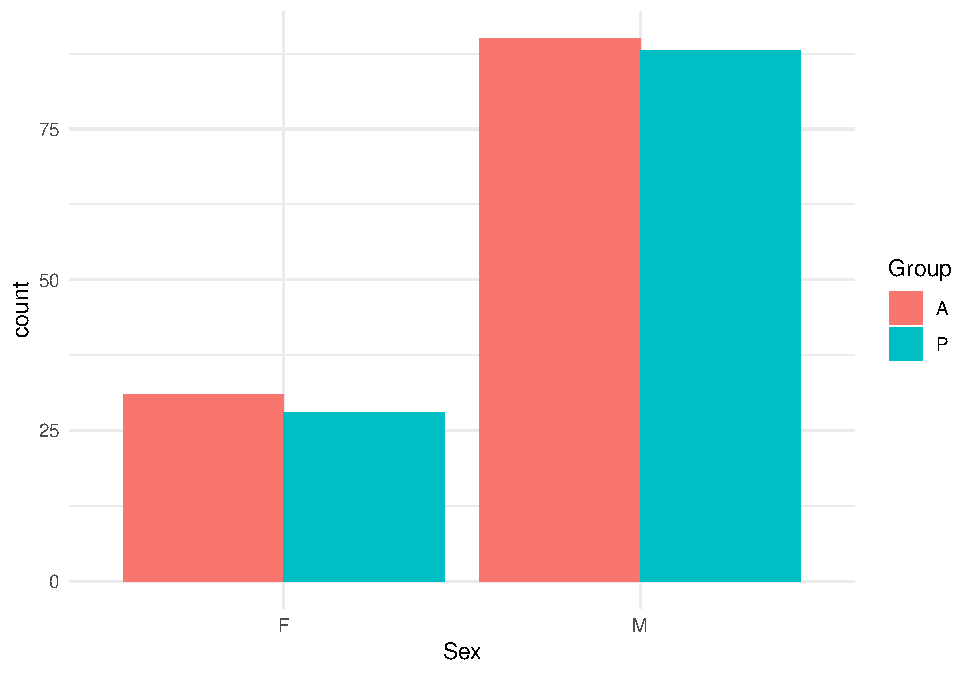
\includegraphics{EDA__files/figure-latex/unnamed-chunk-5-3.pdf}

\begin{Shaded}
\begin{Highlighting}[]
\FunctionTok{ggplot}\NormalTok{(dados\_longos, }\FunctionTok{aes}\NormalTok{(Age, }\AttributeTok{fill =}\NormalTok{ Age }\SpecialCharTok{\textless{}} \DecValTok{50}\NormalTok{)) }\SpecialCharTok{+} 
  \CommentTok{\#geom\_histogram(fill = "yellow", }
  \CommentTok{\#               aes(y = after\_stat(density)), bins=6)+}
  \FunctionTok{geom\_density}\NormalTok{(}\AttributeTok{alpha=}\FloatTok{0.2}\NormalTok{)}\SpecialCharTok{+}
  \FunctionTok{facet\_wrap}\NormalTok{(}\SpecialCharTok{\textasciitilde{}}\NormalTok{Sex)}\SpecialCharTok{+}
  \FunctionTok{theme\_minimal}\NormalTok{()}
\end{Highlighting}
\end{Shaded}

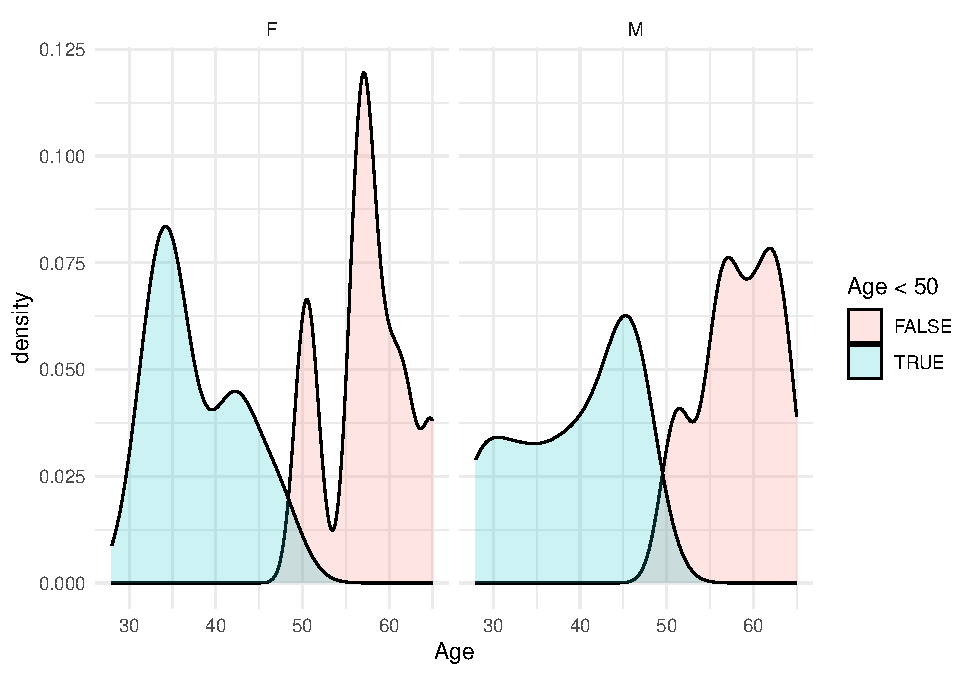
\includegraphics{EDA__files/figure-latex/unnamed-chunk-5-4.pdf}

\hypertarget{transformando-dados-seguindo-o-feito-pelo-jalmar}{%
\subsection{Transformando dados (seguindo o feito pelo
Jalmar)}\label{transformando-dados-seguindo-o-feito-pelo-jalmar}}

\begin{Shaded}
\begin{Highlighting}[]
\NormalTok{dados\_longos}\SpecialCharTok{$}\NormalTok{Sex}\OtherTok{\textless{}{-}} \FunctionTok{recode\_factor}\NormalTok{(dados\_longos}\SpecialCharTok{$}\NormalTok{Sex, }\StringTok{\textasciigrave{}}\AttributeTok{F}\StringTok{\textasciigrave{}} \OtherTok{=} \StringTok{"0"}\NormalTok{, }\StringTok{\textasciigrave{}}\AttributeTok{M}\StringTok{\textasciigrave{}} \OtherTok{=} \StringTok{"1"}\NormalTok{)}

\NormalTok{dados\_longos}\SpecialCharTok{$}\NormalTok{Age}\OtherTok{\textless{}{-}} \FunctionTok{factor}\NormalTok{(}\FunctionTok{case\_when}\NormalTok{(dados\_longos}\SpecialCharTok{$}\NormalTok{Age }\SpecialCharTok{\textless{}}\DecValTok{50}  \SpecialCharTok{\textasciitilde{}} \DecValTok{1}\NormalTok{,}
\NormalTok{  dados\_longos}\SpecialCharTok{$}\NormalTok{Age }\SpecialCharTok{\textgreater{}=}\DecValTok{50} \SpecialCharTok{\textasciitilde{}} \DecValTok{0}\NormalTok{, }\AttributeTok{.default =}\NormalTok{ dados\_longos}\SpecialCharTok{$}\NormalTok{Age), }
  \AttributeTok{levels =} \FunctionTok{c}\NormalTok{(}\DecValTok{0}\NormalTok{, }\DecValTok{1}\NormalTok{))}

\NormalTok{dados\_longos}\SpecialCharTok{$}\NormalTok{Group}\OtherTok{\textless{}{-}} \FunctionTok{recode\_factor}\NormalTok{(dados\_longos}\SpecialCharTok{$}\NormalTok{Group, }\StringTok{\textasciigrave{}}\AttributeTok{P}\StringTok{\textasciigrave{}} \OtherTok{=} \StringTok{"0"}\NormalTok{, }\StringTok{\textasciigrave{}}\AttributeTok{A}\StringTok{\textasciigrave{}} \OtherTok{=} \StringTok{"1"}\NormalTok{)}

\NormalTok{dados\_longos}\SpecialCharTok{$}\NormalTok{week}\OtherTok{\textless{}{-}} \FunctionTok{factor}\NormalTok{(dados\_longos}\SpecialCharTok{$}\NormalTok{week, }
                           \AttributeTok{levels =} \FunctionTok{c}\NormalTok{(}\DecValTok{0}\NormalTok{, }\DecValTok{1}\NormalTok{, }\DecValTok{5}\NormalTok{, }\DecValTok{9}\NormalTok{, }\DecValTok{13}\NormalTok{) )}

\NormalTok{dados\_longos }\SpecialCharTok{\%\textgreater{}\%} 
  \FunctionTok{group\_by}\NormalTok{(week) }\SpecialCharTok{\%\textgreater{}\%} 
  \FunctionTok{summarise}\NormalTok{( }\AttributeTok{n =} \FunctionTok{n}\NormalTok{())}
\end{Highlighting}
\end{Shaded}

\begin{verbatim}
## # A tibble: 5 x 2
##   week      n
##   <fct> <int>
## 1 0        51
## 2 1        51
## 3 5        48
## 4 9        45
## 5 13       42
\end{verbatim}

\hypertarget{gruxe1ficos-de-perfis}{%
\section{Gráficos de perfis}\label{gruxe1ficos-de-perfis}}

\hypertarget{sexo-female-0}{%
\subsection{Sexo Female == 0}\label{sexo-female-0}}

\begin{Shaded}
\begin{Highlighting}[]
\NormalTok{dados\_longos }\SpecialCharTok{\%\textgreater{}\%} \FunctionTok{filter}\NormalTok{(Sex }\SpecialCharTok{==} \StringTok{"0"}\NormalTok{) }\SpecialCharTok{\%\textgreater{}\%}
  \FunctionTok{ggplot}\NormalTok{(}\FunctionTok{aes}\NormalTok{(week, Y, }\AttributeTok{group =}\NormalTok{ id)) }\SpecialCharTok{+}
  \FunctionTok{geom\_point}\NormalTok{()}\SpecialCharTok{+}
  \FunctionTok{geom\_line}\NormalTok{()}\SpecialCharTok{+}
  \FunctionTok{theme\_minimal}\NormalTok{()}\SpecialCharTok{+}
  \FunctionTok{scale\_y\_continuous}\NormalTok{(}\AttributeTok{breaks =} \FunctionTok{c}\NormalTok{(}\DecValTok{0}\NormalTok{,}\DecValTok{1}\NormalTok{))}\SpecialCharTok{+}
  \FunctionTok{facet\_wrap}\NormalTok{(}\SpecialCharTok{\textasciitilde{}}\NormalTok{id)}
\end{Highlighting}
\end{Shaded}

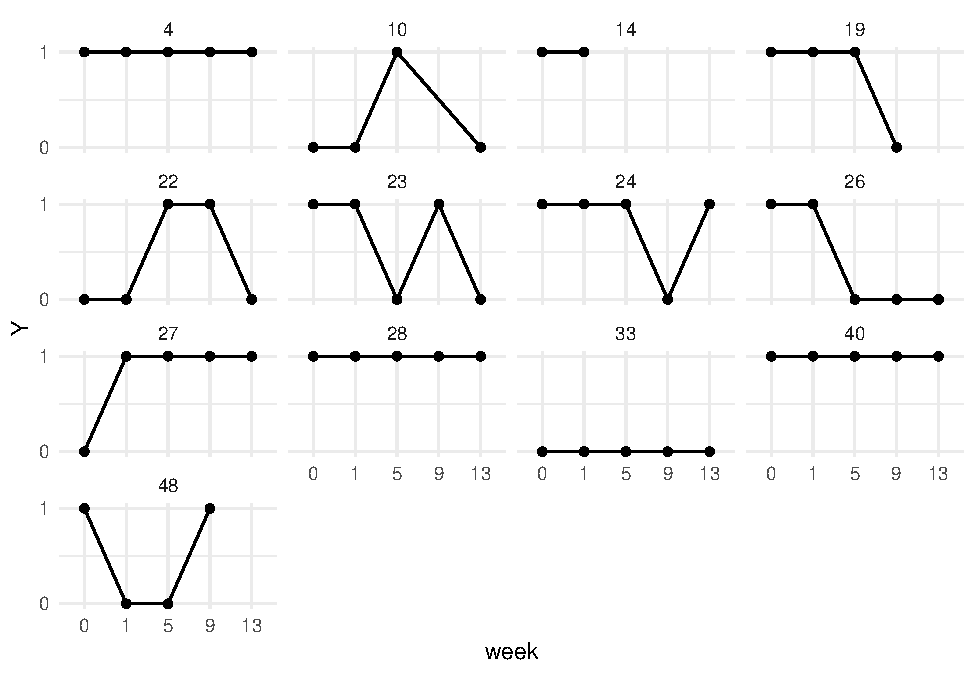
\includegraphics{EDA__files/figure-latex/unnamed-chunk-7-1.pdf}

\hypertarget{sexo-male-1}{%
\subsection{Sexo Male == 1}\label{sexo-male-1}}

\begin{Shaded}
\begin{Highlighting}[]
\NormalTok{dados\_longos }\SpecialCharTok{\%\textgreater{}\%} \FunctionTok{filter}\NormalTok{(Sex }\SpecialCharTok{==} \StringTok{"1"}\NormalTok{) }\SpecialCharTok{\%\textgreater{}\%}
  \FunctionTok{ggplot}\NormalTok{(}\FunctionTok{aes}\NormalTok{(week, Y, }\AttributeTok{group =}\NormalTok{ id)) }\SpecialCharTok{+}
  \FunctionTok{geom\_point}\NormalTok{()}\SpecialCharTok{+}
  \FunctionTok{geom\_line}\NormalTok{()}\SpecialCharTok{+}
  \FunctionTok{theme\_minimal}\NormalTok{()}\SpecialCharTok{+}
  \FunctionTok{scale\_y\_continuous}\NormalTok{(}\AttributeTok{breaks =} \FunctionTok{c}\NormalTok{(}\DecValTok{0}\NormalTok{,}\DecValTok{1}\NormalTok{))}\SpecialCharTok{+}
  \FunctionTok{facet\_wrap}\NormalTok{(}\SpecialCharTok{\textasciitilde{}}\NormalTok{id)}
\end{Highlighting}
\end{Shaded}

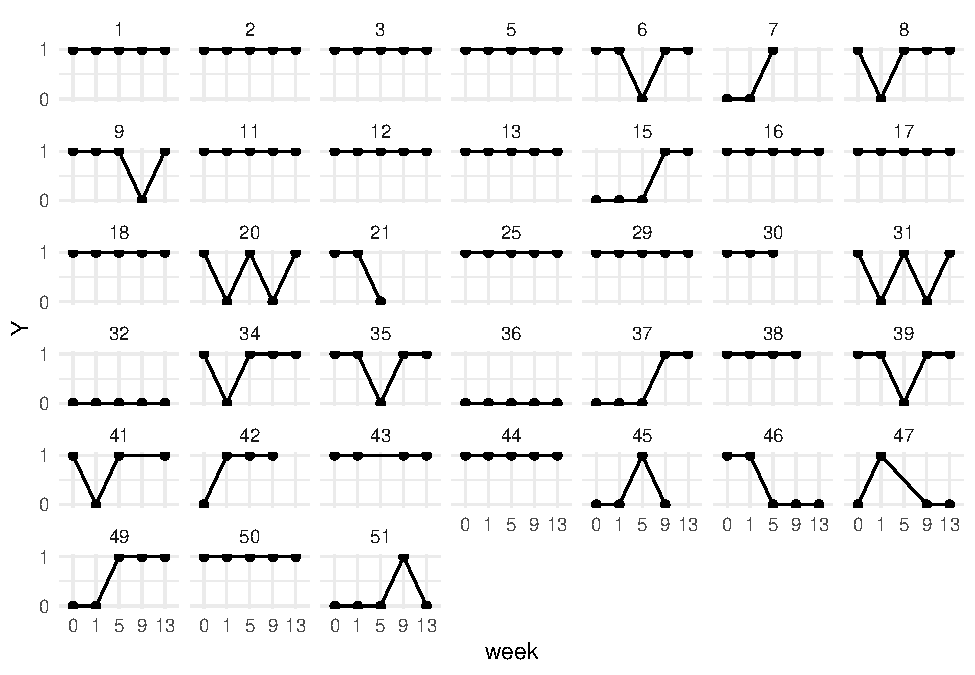
\includegraphics{EDA__files/figure-latex/unnamed-chunk-8-1.pdf}

\hypertarget{ajuste-de-modelos}{%
\section{Ajuste de modelos}\label{ajuste-de-modelos}}

\hypertarget{cloglog}{%
\subsection{cloglog}\label{cloglog}}

\begin{Shaded}
\begin{Highlighting}[]
\NormalTok{modelo\_cloglog}\OtherTok{\textless{}{-}} \FunctionTok{glm}\NormalTok{(Y }\SpecialCharTok{\textasciitilde{}}\NormalTok{ Sex }\SpecialCharTok{+} 
\NormalTok{               Age }\SpecialCharTok{+} 
\NormalTok{               Group }\SpecialCharTok{+} 
               \FunctionTok{as.numeric}\NormalTok{(week),}
             \AttributeTok{family =} \FunctionTok{binomial}\NormalTok{(}\AttributeTok{link =} \StringTok{"cloglog"}\NormalTok{),}
             \AttributeTok{data=}\NormalTok{ dados\_longos)}
\NormalTok{modelo\_cloglog}\SpecialCharTok{$}\NormalTok{family}
\end{Highlighting}
\end{Shaded}

\begin{verbatim}
## 
## Family: binomial 
## Link function: cloglog
\end{verbatim}

\begin{Shaded}
\begin{Highlighting}[]
\FunctionTok{summary}\NormalTok{(modelo\_cloglog)}
\end{Highlighting}
\end{Shaded}

\begin{verbatim}
## 
## Call:
## glm(formula = Y ~ Sex + Age + Group + as.numeric(week), family = binomial(link = "cloglog"), 
##     data = dados_longos)
## 
## Deviance Residuals: 
##     Min       1Q   Median       3Q      Max  
## -2.0202  -1.2688   0.6394   0.8721   1.2010  
## 
## Coefficients:
##                  Estimate Std. Error z value Pr(>|z|)    
## (Intercept)      -0.46985    0.27391  -1.715 0.086281 .  
## Sex1              0.29448    0.19859   1.483 0.138115    
## Age1              0.05639    0.17402   0.324 0.745898    
## Group1            0.57257    0.16874   3.393 0.000691 ***
## as.numeric(week)  0.06321    0.05979   1.057 0.290470    
## ---
## Signif. codes:  0 '***' 0.001 '**' 0.01 '*' 0.05 '.' 0.1 ' ' 1
## 
## (Dispersion parameter for binomial family taken to be 1)
## 
##     Null deviance: 282.26  on 236  degrees of freedom
## Residual deviance: 268.18  on 232  degrees of freedom
## AIC: 278.18
## 
## Number of Fisher Scoring iterations: 5
\end{verbatim}

\begin{Shaded}
\begin{Highlighting}[]
\FunctionTok{hnp}\NormalTok{(modelo\_cloglog, }\AttributeTok{print.on =} \ConstantTok{TRUE}\NormalTok{)}
\end{Highlighting}
\end{Shaded}

\begin{verbatim}
## Binomial model
\end{verbatim}

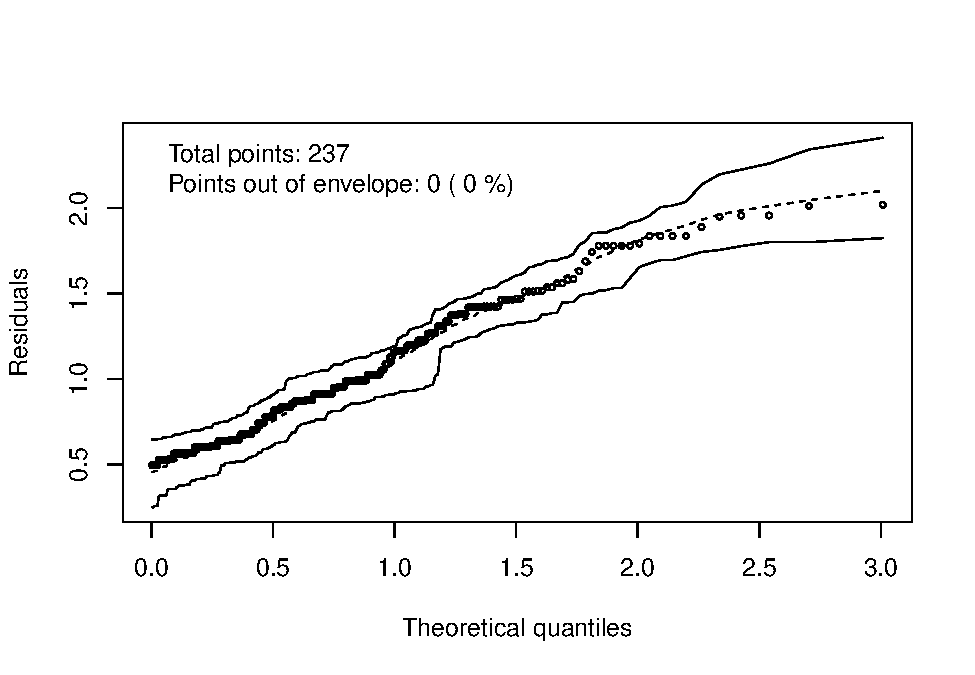
\includegraphics{EDA__files/figure-latex/unnamed-chunk-9-1.pdf}

\begin{Shaded}
\begin{Highlighting}[]
\FunctionTok{plot}\NormalTok{(}\FunctionTok{predict.glm}\NormalTok{(modelo\_cloglog, }\AttributeTok{type=}\StringTok{"response"}\NormalTok{)}\SpecialCharTok{\textasciitilde{}}\FunctionTok{predict.glm}\NormalTok{(modelo\_cloglog, }\AttributeTok{type=}\StringTok{"link"}\NormalTok{),}
     \AttributeTok{ylab =} \StringTok{"Probabilidades"}\NormalTok{,}
     \AttributeTok{xlab =}  \StringTok{"modelo cloglog"}\NormalTok{,}
     \AttributeTok{ylim=}\FunctionTok{c}\NormalTok{(}\DecValTok{0}\NormalTok{,}\DecValTok{1}\NormalTok{))}
\end{Highlighting}
\end{Shaded}

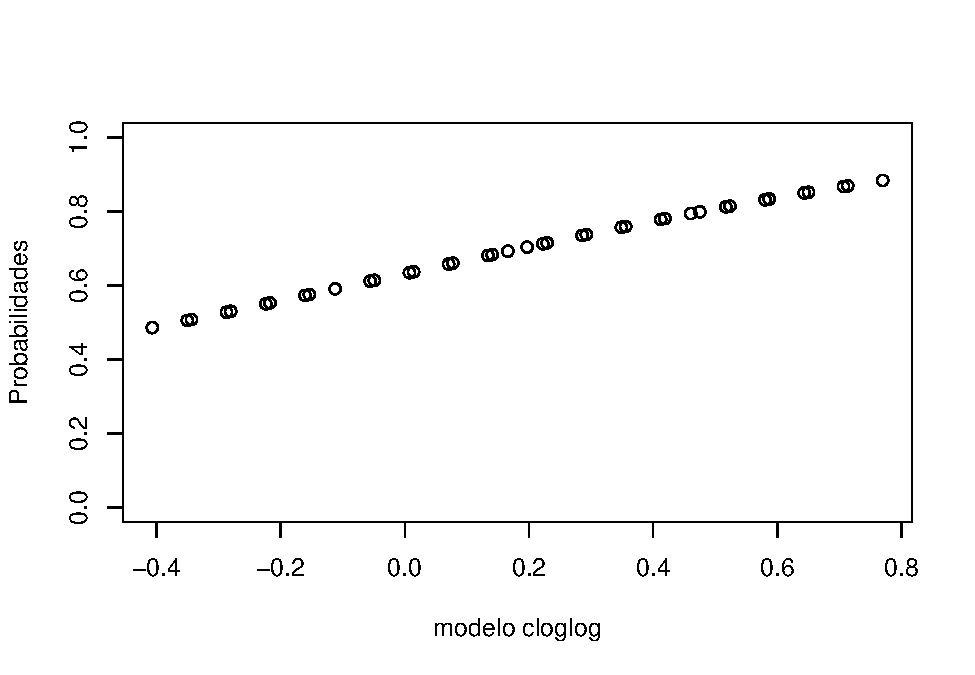
\includegraphics{EDA__files/figure-latex/unnamed-chunk-9-2.pdf}

\hypertarget{logit}{%
\subsection{logit}\label{logit}}

\begin{Shaded}
\begin{Highlighting}[]
\NormalTok{modelo\_logit}\OtherTok{\textless{}{-}} \FunctionTok{glm}\NormalTok{(Y }\SpecialCharTok{\textasciitilde{}}\NormalTok{ Sex }\SpecialCharTok{+} 
\NormalTok{               Age }\SpecialCharTok{+} 
\NormalTok{               Group }\SpecialCharTok{+} 
               \FunctionTok{as.numeric}\NormalTok{(week),}
                     \AttributeTok{family =} \FunctionTok{binomial}\NormalTok{(}\AttributeTok{link =} \StringTok{"logit"}\NormalTok{),}
                     \AttributeTok{data=}\NormalTok{ dados\_longos)}
\NormalTok{modelo\_logit}\SpecialCharTok{$}\NormalTok{family}
\end{Highlighting}
\end{Shaded}

\begin{verbatim}
## 
## Family: binomial 
## Link function: logit
\end{verbatim}

\begin{Shaded}
\begin{Highlighting}[]
\FunctionTok{summary}\NormalTok{(modelo\_logit)}
\end{Highlighting}
\end{Shaded}

\begin{verbatim}
## 
## Call:
## glm(formula = Y ~ Sex + Age + Group + as.numeric(week), family = binomial(link = "logit"), 
##     data = dados_longos)
## 
## Deviance Residuals: 
##     Min       1Q   Median       3Q      Max  
## -1.9579  -1.2612   0.6309   0.8723   1.1986  
## 
## Coefficients:
##                  Estimate Std. Error z value Pr(>|z|)   
## (Intercept)      -0.13114    0.44776  -0.293  0.76962   
## Sex1              0.49379    0.33640   1.468  0.14214   
## Age1              0.03550    0.31166   0.114  0.90930   
## Group1            0.98760    0.30382   3.251  0.00115 **
## as.numeric(week)  0.08148    0.10635   0.766  0.44360   
## ---
## Signif. codes:  0 '***' 0.001 '**' 0.01 '*' 0.05 '.' 0.1 ' ' 1
## 
## (Dispersion parameter for binomial family taken to be 1)
## 
##     Null deviance: 282.26  on 236  degrees of freedom
## Residual deviance: 268.79  on 232  degrees of freedom
## AIC: 278.79
## 
## Number of Fisher Scoring iterations: 4
\end{verbatim}

\begin{Shaded}
\begin{Highlighting}[]
\FunctionTok{hnp}\NormalTok{(modelo\_logit, }\AttributeTok{print.on =} \ConstantTok{TRUE}\NormalTok{)}
\end{Highlighting}
\end{Shaded}

\begin{verbatim}
## Binomial model
\end{verbatim}

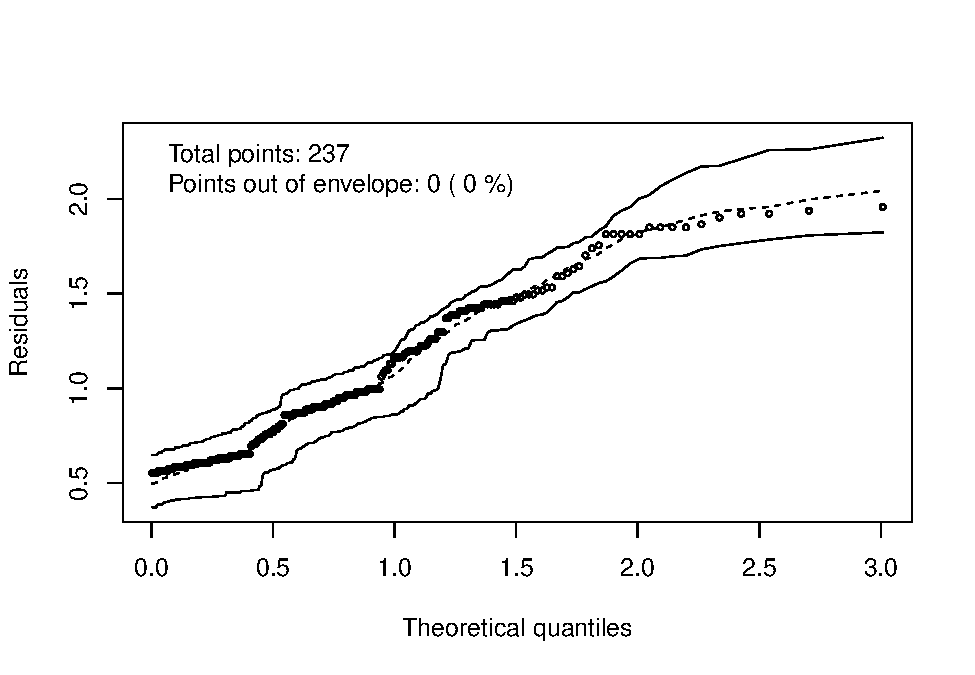
\includegraphics{EDA__files/figure-latex/unnamed-chunk-10-1.pdf}

\begin{Shaded}
\begin{Highlighting}[]
\FunctionTok{plot}\NormalTok{(}\FunctionTok{predict.glm}\NormalTok{(modelo\_logit, }\AttributeTok{type=}\StringTok{"response"}\NormalTok{)}\SpecialCharTok{\textasciitilde{}}\FunctionTok{predict.glm}\NormalTok{(modelo\_logit, }\AttributeTok{type=}\StringTok{"link"}\NormalTok{),}
     \AttributeTok{ylab =} \StringTok{"Probabilidades"}\NormalTok{,}
     \AttributeTok{xlab =}  \StringTok{"modelo logit"}\NormalTok{,}
     \AttributeTok{ylim=}\FunctionTok{c}\NormalTok{(}\DecValTok{0}\NormalTok{,}\DecValTok{1}\NormalTok{))}
\end{Highlighting}
\end{Shaded}

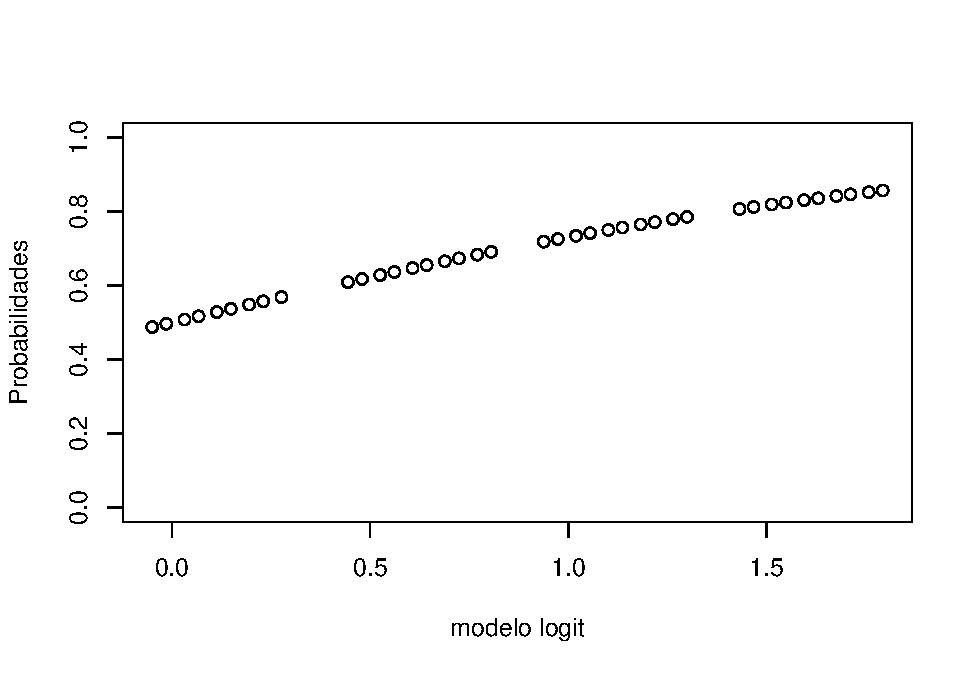
\includegraphics{EDA__files/figure-latex/unnamed-chunk-10-2.pdf}

\hypertarget{probit}{%
\subsection{probit}\label{probit}}

\begin{Shaded}
\begin{Highlighting}[]
\NormalTok{modelo\_probit}\OtherTok{\textless{}{-}} \FunctionTok{glm}\NormalTok{(Y }\SpecialCharTok{\textasciitilde{}}\NormalTok{ Sex }\SpecialCharTok{+} 
\NormalTok{               Age }\SpecialCharTok{+} 
\NormalTok{               Group }\SpecialCharTok{+} 
               \FunctionTok{as.numeric}\NormalTok{(week),}
                   \AttributeTok{family =} \FunctionTok{binomial}\NormalTok{(}\AttributeTok{link =} \StringTok{"probit"}\NormalTok{),}
                   \AttributeTok{data=}\NormalTok{ dados\_longos)}
\NormalTok{modelo\_probit}\SpecialCharTok{$}\NormalTok{family}
\end{Highlighting}
\end{Shaded}

\begin{verbatim}
## 
## Family: binomial 
## Link function: probit
\end{verbatim}

\begin{Shaded}
\begin{Highlighting}[]
\FunctionTok{summary}\NormalTok{(modelo\_probit)}
\end{Highlighting}
\end{Shaded}

\begin{verbatim}
## 
## Call:
## glm(formula = Y ~ Sex + Age + Group + as.numeric(week), family = binomial(link = "probit"), 
##     data = dados_longos)
## 
## Deviance Residuals: 
##     Min       1Q   Median       3Q      Max  
## -1.9750  -1.2650   0.6329   0.8721   1.2001  
## 
## Coefficients:
##                  Estimate Std. Error z value Pr(>|z|)    
## (Intercept)      -0.08693    0.27115  -0.321 0.748510    
## Sex1              0.29695    0.20235   1.468 0.142233    
## Age1              0.03294    0.18530   0.178 0.858905    
## Group1            0.59240    0.17866   3.316 0.000914 ***
## as.numeric(week)  0.05359    0.06329   0.847 0.397121    
## ---
## Signif. codes:  0 '***' 0.001 '**' 0.01 '*' 0.05 '.' 0.1 ' ' 1
## 
## (Dispersion parameter for binomial family taken to be 1)
## 
##     Null deviance: 282.26  on 236  degrees of freedom
## Residual deviance: 268.63  on 232  degrees of freedom
## AIC: 278.63
## 
## Number of Fisher Scoring iterations: 4
\end{verbatim}

\begin{Shaded}
\begin{Highlighting}[]
\FunctionTok{hnp}\NormalTok{(modelo\_probit, }\AttributeTok{print.on =} \ConstantTok{TRUE}\NormalTok{)}
\end{Highlighting}
\end{Shaded}

\begin{verbatim}
## Binomial model
\end{verbatim}

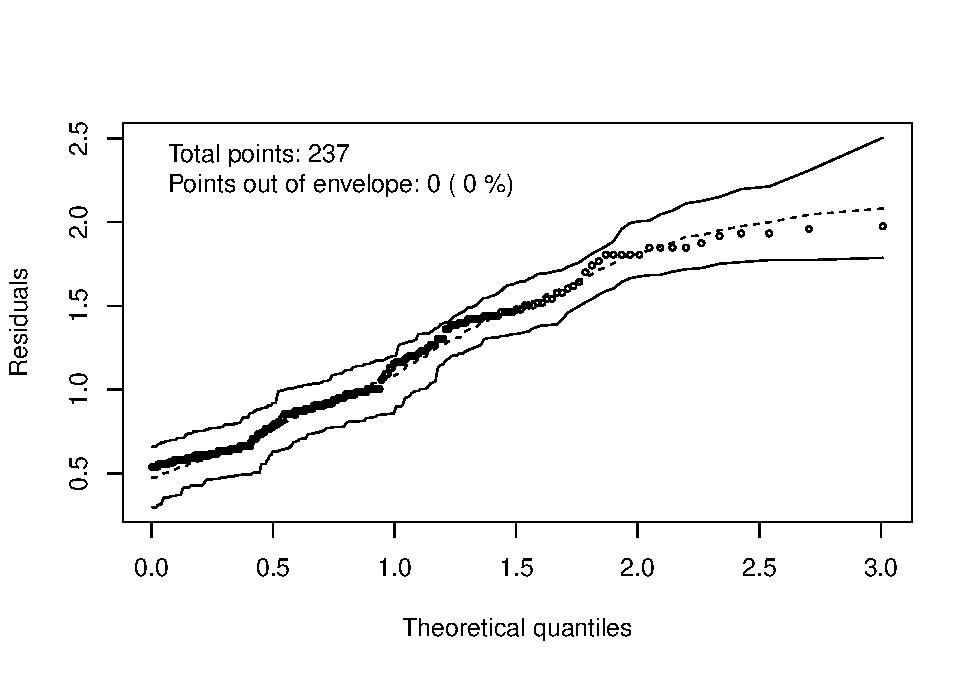
\includegraphics{EDA__files/figure-latex/unnamed-chunk-11-1.pdf}

\begin{Shaded}
\begin{Highlighting}[]
\FunctionTok{plot}\NormalTok{(}\FunctionTok{predict.glm}\NormalTok{(modelo\_probit, }\AttributeTok{type=}\StringTok{"response"}\NormalTok{)}\SpecialCharTok{\textasciitilde{}}\FunctionTok{predict.glm}\NormalTok{(modelo\_probit, }\AttributeTok{type=}\StringTok{"link"}\NormalTok{),}
     \AttributeTok{ylab =} \StringTok{"Probabilidades"}\NormalTok{,}
     \AttributeTok{xlab =} \StringTok{"modelo probit"}\NormalTok{,}
     \AttributeTok{ylim=}\FunctionTok{c}\NormalTok{(}\DecValTok{0}\NormalTok{,}\DecValTok{1}\NormalTok{))}
\end{Highlighting}
\end{Shaded}

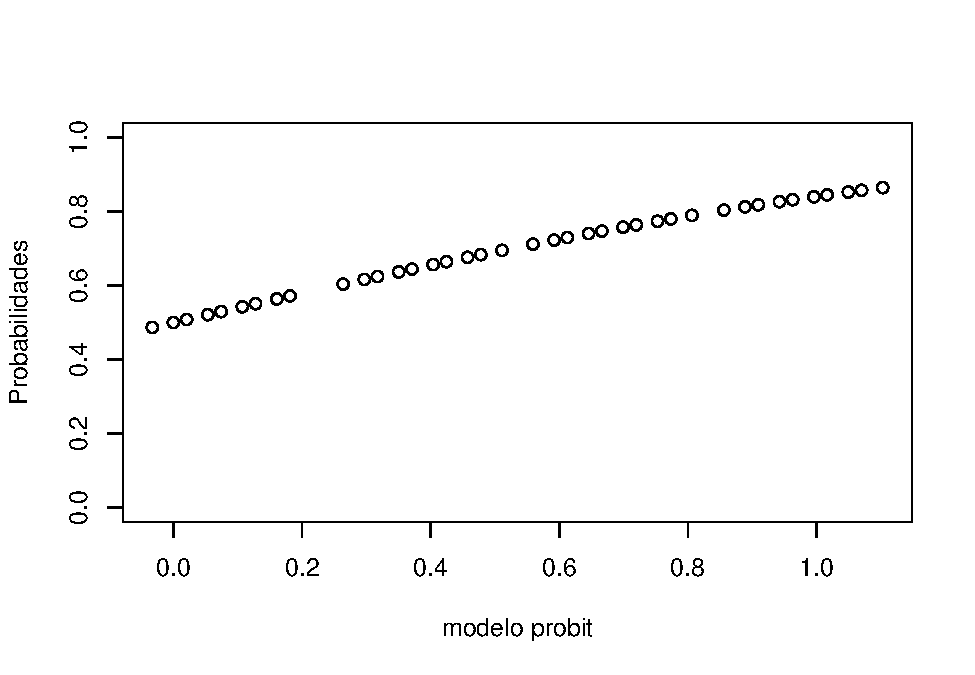
\includegraphics{EDA__files/figure-latex/unnamed-chunk-11-2.pdf}

\hypertarget{cauchit}{%
\subsection{cauchit}\label{cauchit}}

\begin{Shaded}
\begin{Highlighting}[]
\NormalTok{modelo\_cauchit}\OtherTok{\textless{}{-}} \FunctionTok{glm}\NormalTok{(Y }\SpecialCharTok{\textasciitilde{}}\NormalTok{ Sex }\SpecialCharTok{+} 
\NormalTok{               Age }\SpecialCharTok{+} 
\NormalTok{               Group }\SpecialCharTok{+} 
               \FunctionTok{as.numeric}\NormalTok{(week),}
                    \AttributeTok{family =} \FunctionTok{binomial}\NormalTok{(}\AttributeTok{link =} \StringTok{"cauchit"}\NormalTok{),}
                    \AttributeTok{data=}\NormalTok{ dados\_longos)}
\NormalTok{modelo\_cauchit}\SpecialCharTok{$}\NormalTok{family}
\end{Highlighting}
\end{Shaded}

\begin{verbatim}
## 
## Family: binomial 
## Link function: cauchit
\end{verbatim}

\begin{Shaded}
\begin{Highlighting}[]
\FunctionTok{summary}\NormalTok{(modelo\_cauchit)}
\end{Highlighting}
\end{Shaded}

\begin{verbatim}
## 
## Call:
## glm(formula = Y ~ Sex + Age + Group + as.numeric(week), family = binomial(link = "cauchit"), 
##     data = dados_longos)
## 
## Deviance Residuals: 
##     Min       1Q   Median       3Q      Max  
## -1.8815  -1.2323   0.6286   0.8943   1.2118  
## 
## Coefficients:
##                   Estimate Std. Error z value Pr(>|z|)   
## (Intercept)      -0.002309   0.420176  -0.005   0.9956   
## Sex1              0.492029   0.334590   1.471   0.1414   
## Age1             -0.086834   0.321406  -0.270   0.7870   
## Group1            1.068118   0.383931   2.782   0.0054 **
## as.numeric(week)  0.025811   0.107747   0.240   0.8107   
## ---
## Signif. codes:  0 '***' 0.001 '**' 0.01 '*' 0.05 '.' 0.1 ' ' 1
## 
## (Dispersion parameter for binomial family taken to be 1)
## 
##     Null deviance: 282.26  on 236  degrees of freedom
## Residual deviance: 269.49  on 232  degrees of freedom
## AIC: 279.49
## 
## Number of Fisher Scoring iterations: 6
\end{verbatim}

\begin{Shaded}
\begin{Highlighting}[]
\FunctionTok{hnp}\NormalTok{(modelo\_cauchit, }\AttributeTok{print.on =} \ConstantTok{TRUE}\NormalTok{)}
\end{Highlighting}
\end{Shaded}

\begin{verbatim}
## Binomial model
\end{verbatim}

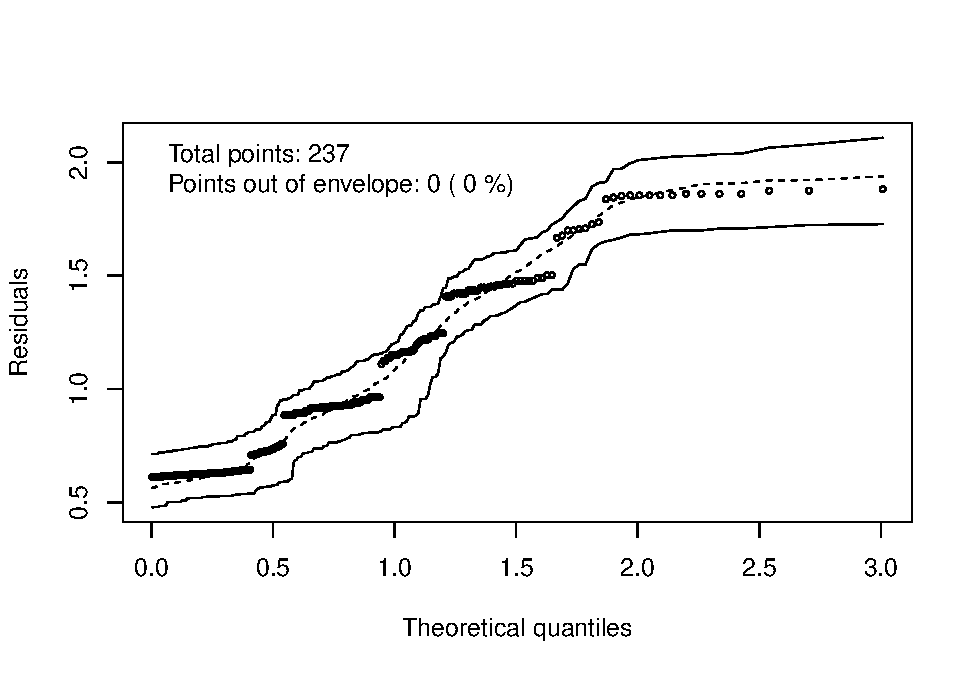
\includegraphics{EDA__files/figure-latex/unnamed-chunk-12-1.pdf}

\begin{Shaded}
\begin{Highlighting}[]
\FunctionTok{plot}\NormalTok{(}\FunctionTok{predict.glm}\NormalTok{(modelo\_cauchit, }\AttributeTok{type=}\StringTok{"response"}\NormalTok{)}\SpecialCharTok{\textasciitilde{}}\FunctionTok{predict.glm}\NormalTok{(modelo\_cauchit, }\AttributeTok{type=}\StringTok{"link"}\NormalTok{),}
     \AttributeTok{ylab =} \StringTok{"Probabilidades"}\NormalTok{,}
     \AttributeTok{xlab =}  \StringTok{"modelo cauchit"}\NormalTok{,}
     \AttributeTok{ylim=}\FunctionTok{c}\NormalTok{(}\DecValTok{0}\NormalTok{,}\DecValTok{1}\NormalTok{))}
\end{Highlighting}
\end{Shaded}

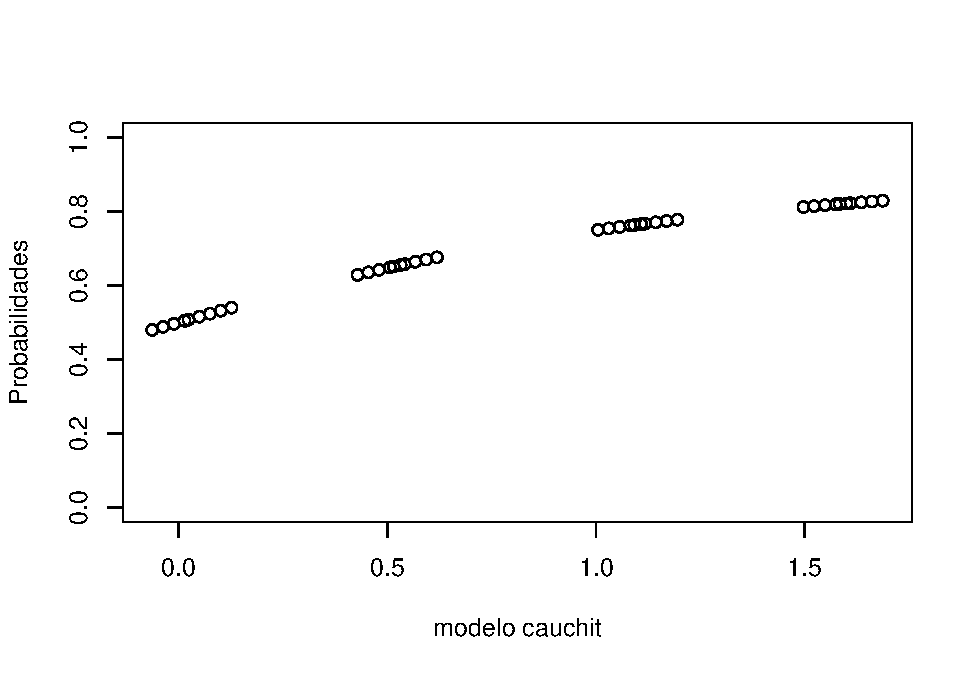
\includegraphics{EDA__files/figure-latex/unnamed-chunk-12-2.pdf}

\hypertarget{gee}{%
\section{GEE}\label{gee}}

\hypertarget{independence}{%
\subsection{independence}\label{independence}}

\begin{Shaded}
\begin{Highlighting}[]
\FunctionTok{library}\NormalTok{(gee) }
\NormalTok{modelo\_gee\_1 }\OtherTok{\textless{}{-}} \FunctionTok{gee}\NormalTok{(Y }\SpecialCharTok{\textasciitilde{}}\NormalTok{ Sex }\SpecialCharTok{+}\NormalTok{ Age }\SpecialCharTok{+}\NormalTok{ Group }\SpecialCharTok{+} \FunctionTok{as.numeric}\NormalTok{(week), }
               \AttributeTok{data =}\NormalTok{ dados\_longos, }
               \AttributeTok{id =}\NormalTok{ id, }
               \AttributeTok{family =} \FunctionTok{binomial}\NormalTok{(}\AttributeTok{link =} \StringTok{"cloglog"}\NormalTok{),}
               \AttributeTok{corstr =} \StringTok{"independence"}\NormalTok{)}
\end{Highlighting}
\end{Shaded}

\begin{verbatim}
##      (Intercept)             Sex1             Age1           Group1 
##      -0.46985374       0.29447851       0.05639087       0.57257244 
## as.numeric(week) 
##       0.06320692
\end{verbatim}

\begin{Shaded}
\begin{Highlighting}[]
\FunctionTok{summary}\NormalTok{(modelo\_gee\_1)}
\end{Highlighting}
\end{Shaded}

\begin{verbatim}
## 
##  GEE:  GENERALIZED LINEAR MODELS FOR DEPENDENT DATA
##  gee S-function, version 4.13 modified 98/01/27 (1998) 
## 
## Model:
##  Link:                      Cloglog 
##  Variance to Mean Relation: Binomial 
##  Correlation Structure:     Independent 
## 
## Call:
## gee(formula = Y ~ Sex + Age + Group + as.numeric(week), id = id, 
##     data = dados_longos, family = binomial(link = "cloglog"), 
##     corstr = "independence")
## 
## Summary of Residuals:
##        Min         1Q     Median         3Q        Max 
## -0.8700482 -0.5528727  0.1848709  0.3163075  0.5138260 
## 
## 
## Coefficients:
##                     Estimate Naive S.E.   Naive z Robust S.E.   Robust z
## (Intercept)      -0.46987242  0.2760654 -1.702033  0.32613496 -1.4407300
## Sex1              0.29447626  0.2001501  1.471277  0.27987872  1.0521567
## Age1              0.05640169  0.1753833  0.321591  0.24953232  0.2260296
## Group1            0.57257352  0.1700686  3.366721  0.24311673  2.3551383
## as.numeric(week)  0.06321248  0.0602626  1.048950  0.05275103  1.1983173
## 
## Estimated Scale Parameter:  1.015735
## Number of Iterations:  1
## 
## Working Correlation
##      [,1] [,2] [,3] [,4] [,5]
## [1,]    1    0    0    0    0
## [2,]    0    1    0    0    0
## [3,]    0    0    1    0    0
## [4,]    0    0    0    1    0
## [5,]    0    0    0    0    1
\end{verbatim}

\hypertarget{exchangeable}{%
\subsection{exchangeable}\label{exchangeable}}

\begin{Shaded}
\begin{Highlighting}[]
\NormalTok{modelo\_gee\_2 }\OtherTok{\textless{}{-}} \FunctionTok{gee}\NormalTok{(Y }\SpecialCharTok{\textasciitilde{}}\NormalTok{ Sex }\SpecialCharTok{+}\NormalTok{ Age }\SpecialCharTok{+}\NormalTok{ Group }\SpecialCharTok{+} \FunctionTok{as.numeric}\NormalTok{(week), }
               \AttributeTok{data =}\NormalTok{ dados\_longos, }
               \AttributeTok{id =}\NormalTok{ id, }
               \AttributeTok{family =} \FunctionTok{binomial}\NormalTok{(}\AttributeTok{link =} \StringTok{"cloglog"}\NormalTok{),}
               \AttributeTok{corstr =} \StringTok{"exchangeable"}\NormalTok{)}
\end{Highlighting}
\end{Shaded}

\begin{verbatim}
##      (Intercept)             Sex1             Age1           Group1 
##      -0.46985374       0.29447851       0.05639087       0.57257244 
## as.numeric(week) 
##       0.06320692
\end{verbatim}

\begin{Shaded}
\begin{Highlighting}[]
\FunctionTok{summary}\NormalTok{(modelo\_gee\_2)}
\end{Highlighting}
\end{Shaded}

\begin{verbatim}
## 
##  GEE:  GENERALIZED LINEAR MODELS FOR DEPENDENT DATA
##  gee S-function, version 4.13 modified 98/01/27 (1998) 
## 
## Model:
##  Link:                      Cloglog 
##  Variance to Mean Relation: Binomial 
##  Correlation Structure:     Exchangeable 
## 
## Call:
## gee(formula = Y ~ Sex + Age + Group + as.numeric(week), id = id, 
##     data = dados_longos, family = binomial(link = "cloglog"), 
##     corstr = "exchangeable")
## 
## Summary of Residuals:
##        Min         1Q     Median         3Q        Max 
## -0.8599897 -0.5530691  0.1870639  0.3276707  0.5032505 
## 
## 
## Coefficients:
##                     Estimate Naive S.E.    Naive z Robust S.E.   Robust z
## (Intercept)      -0.42904864 0.33365054 -1.2859222  0.32034671 -1.3393259
## Sex1              0.27285705 0.28277327  0.9649323  0.27849472  0.9797567
## Age1              0.08134966 0.24774357  0.3283623  0.24724658  0.3290224
## Group1            0.53829103 0.24201844  2.2241736  0.24310512  2.2142316
## as.numeric(week)  0.05314300 0.05066053  1.0490021  0.05083011  1.0455023
## 
## Estimated Scale Parameter:  0.9965314
## Number of Iterations:  4
## 
## Working Correlation
##           [,1]      [,2]      [,3]      [,4]      [,5]
## [1,] 1.0000000 0.2907233 0.2907233 0.2907233 0.2907233
## [2,] 0.2907233 1.0000000 0.2907233 0.2907233 0.2907233
## [3,] 0.2907233 0.2907233 1.0000000 0.2907233 0.2907233
## [4,] 0.2907233 0.2907233 0.2907233 1.0000000 0.2907233
## [5,] 0.2907233 0.2907233 0.2907233 0.2907233 1.0000000
\end{verbatim}

\hypertarget{unstructured}{%
\subsection{unstructured}\label{unstructured}}

\begin{Shaded}
\begin{Highlighting}[]
\NormalTok{modelo\_gee\_3 }\OtherTok{\textless{}{-}} \FunctionTok{gee}\NormalTok{(Y }\SpecialCharTok{\textasciitilde{}}\NormalTok{ Sex }\SpecialCharTok{+}\NormalTok{ Age }\SpecialCharTok{+}\NormalTok{ Group }\SpecialCharTok{+} \FunctionTok{as.numeric}\NormalTok{(week), }
               \AttributeTok{data =}\NormalTok{ dados\_longos, }
               \AttributeTok{id =}\NormalTok{ id, }
               \AttributeTok{family =} \FunctionTok{binomial}\NormalTok{(}\AttributeTok{link =} \StringTok{"cloglog"}\NormalTok{),}
               \AttributeTok{corstr =} \StringTok{"unstructured"}\NormalTok{)}
\end{Highlighting}
\end{Shaded}

\begin{verbatim}
##      (Intercept)             Sex1             Age1           Group1 
##      -0.46985374       0.29447851       0.05639087       0.57257244 
## as.numeric(week) 
##       0.06320692
\end{verbatim}

\begin{Shaded}
\begin{Highlighting}[]
\FunctionTok{summary}\NormalTok{(modelo\_gee\_3)}
\end{Highlighting}
\end{Shaded}

\begin{verbatim}
## 
##  GEE:  GENERALIZED LINEAR MODELS FOR DEPENDENT DATA
##  gee S-function, version 4.13 modified 98/01/27 (1998) 
## 
## Model:
##  Link:                      Cloglog 
##  Variance to Mean Relation: Binomial 
##  Correlation Structure:     Unstructured 
## 
## Call:
## gee(formula = Y ~ Sex + Age + Group + as.numeric(week), id = id, 
##     data = dados_longos, family = binomial(link = "cloglog"), 
##     corstr = "unstructured")
## 
## Summary of Residuals:
##        Min         1Q     Median         3Q        Max 
## -0.8703654 -0.5230487  0.1650142  0.3603214  0.5205362 
## 
## 
## Coefficients:
##                      Estimate Naive S.E.     Naive z Robust S.E.    Robust z
## (Intercept)      -0.468235192  0.3394253 -1.37949401  0.32501737 -1.44064666
## Sex1              0.279293127  0.2731156  1.02261888  0.27175387  1.02774297
## Age1              0.007621797  0.2397362  0.03179243  0.24396340  0.03124156
## Group1            0.693890430  0.2333050  2.97417687  0.24223920  2.86448444
## as.numeric(week)  0.041897668  0.0552891  0.75779257  0.04990972  0.83946913
## 
## Estimated Scale Parameter:  1.028027
## Number of Iterations:  7
## 
## Working Correlation
##           [,1]       [,2]       [,3]      [,4]      [,5]
## [1,] 1.0000000 0.64699683 0.19879899 0.3105900 0.2345909
## [2,] 0.6469968 1.00000000 0.02545539 0.2919917 0.1593287
## [3,] 0.1987990 0.02545539 1.00000000 0.1337962 0.2364074
## [4,] 0.3105900 0.29199173 0.13379622 1.0000000 0.1851979
## [5,] 0.2345909 0.15932868 0.23640737 0.1851979 1.0000000
\end{verbatim}

\end{document}
